\documentclass[pdflatex,a4paper,11pt,titlepage]{article}

%% Load packages ========================================
\usepackage[T1]{fontenc}

\usepackage{xr-hyper} % Needs to be loaded before hyperref
\usepackage{ifpdf,ifxetex}
\ifxetex
  \usepackage{epstopdf}
  \epstopdfsetup{suffix=.\SourceExt}
  \usepackage{fontspec}           % XeLaTeX specific
  \defaultfontfeatures{Mapping=tex-text} % For archaic input (e.g. convert -- to en-dash)
  \setmainfont{Linux Libertine O}  % LaTeX default (Computer Modern Unicode)
  \usepackage[xetex,colorlinks,unicode=True]{hyperref}
\else
  \usepackage[utf8]{inputenc}     % support utf8 (if possible: use xetex)
  \usepackage{lmodern}
  \usepackage{newunicodechar}
  \ifpdf
    \usepackage[pdftex]{graphicx}
    \usepackage{epstopdf}
    \epstopdfsetup{suffix=.\SourceExt}
    \usepackage[pdftex,colorlinks,unicode=True]{hyperref}
  \else
    \usepackage{graphicx}
    \usepackage[colorlinks,unicode=True]{hyperref}
  \fi
\fi
\usepackage[dvipsnames]{xcolor}
\usepackage{subfig}

\usepackage{booktabs} % <--- This is the way to do it if you ask me.

\usepackage[absolute,overlay]{textpos} % textblock (see inc/kth_titlepage)

\usepackage{authblk}
\renewcommand\Authsep{, }
\renewcommand\Authand{ och }
\renewcommand\Authands{, och }
%\renewcommand*{\thefootnote}{\fnsymbol{footnote}}
\usepackage[perpage]{footmisc} % \cite => numbers
\renewcommand{\thefootnote}{\fnsymbol{footnote}}
\usepackage[style=chem-acs,doi,autocite=superscript,pageranges=false,backend=biber]{biblatex}
\AtEveryBibitem{\clearfield{month}} % Don't put "Jan. 2000" in references
\AtEveryCitekey{\clearfield{month}} % http://tex.stackexchange.com/questions/55780
\renewcommand{\cite}{\autocite}
\usepackage{amsmath, amsfonts, amssymb, amsthm}
\usepackage{siunitx}
\DeclareSIUnit\molar{\mole\per\cubic\deci\metre}
\DeclareSIUnit\Molar{\textsc{m}}
\usepackage[version=3]{mhchem}
%\usepackage{chemstyle}  % \standardstate symbol
\newcommand*{\plimsoll}{{\ensuremath{-\kern-5pt{\circ}\kern-5pt-}}} % standard state symbol

% Make References appear in Table of Contents
\usepackage[nottoc,notlof,notlot,numbib]{tocbibind}

\hypersetup{%
  bookmarksnumbered=true, %
  breaklinks=false, %
  raiselinks=true, %
  pdfborder={0 0 0}, %
  colorlinks=true, %
  plainpages=false, %
  pdfstartview={FitH}, %
  pdfcreator={LaTeX with hyperref package}, %
  citecolor=teal, % See xcolor package documentation
  linkcolor=Maroon, %
  urlcolor=blue, %
}%

\input{derivations/symbnames}
\addbibresource{main.bib}

\externaldocument{supp_mater}

\usepackage[absolute,overlay]{textpos}

%% Global Last Commands
\usepackage[capitalise,noabbrev,swedish]{cleveref} % Needs to be loaded late (see doc)

\providecommand{\projecttitle}{Laborationshandledning -- Stopped flow \\
KD1080}
\hypersetup{%
  pdfkeywords={stopped flow},%
  pdfauthor={Björn Dahlgren},%
  pdftitle={KD1080 \projecttitle}%
}
\providecommand{\mailto}{\texttt{\href{mailto:bda@kth.se}{bda@kth.se}}}
\author[1]{Björn Dahlgren (\mailto)}
\affil[1]{School of Chemical Science and Engineering, Applied Physical Chemistry, KTH}

\title{\projecttitle}


\begin{document}

\makeatletter
    \begin{titlepage}
\begin{textblock*}{2cm}(12mm,12mm) % {block width} (coords)

\includegraphics[width=2cm]{fig/kth.pdf}
\end{textblock*}
      % \begin{picture}(1,1)
      %   \put(0,0){\hbox{
\includegraphics[width=2cm]{fig/kth.pdf}}}
      % \end{picture}
      \begin{center}
        ~\\[20ex]
            {\LARGE \bfseries \sffamily \@title }\\[4ex]
            {\Large  \@author}\\[4ex]
            \@date \\[14ex]
            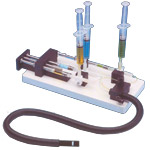
\includegraphics[width=4cm]{fig/setup.jpg}
        \end{center}
    \end{titlepage}
\makeatother
\thispagestyle{empty}
\newpage

%Add content for page two here (useful for two-sided printing)
\thispagestyle{empty}
\newpage

% \maketitle
\setcounter{page}{1} %Start the actually document on page 1

  \tableofcontents
  \listoffigures
  \listoftables
  \pagebreak

  \setlength{\parindent}{0em}
  \setlength{\parskip}{1em}

  \section{Inledning}
\label{sec:inledning}
I denna laboration skall ni, i vattenlösning, studera hastigheten för
(framåt-) reaktionen mellan järn(III)joner och tiocyanatjoner:

\begin{center}
\begin{tabular}{ccc}
  \ce{Fe^3+ + SCN- <=>>[k_f][k_b] FeSCN^2+} & %
    $\log_{10} \left( \beta_1 %
     % (I=\SIrange{1.0}{1.2}{\molar}) %
    / \si{\per\Molar} \right) = \num{2.065(5)}$ %
  % & $\Delta H_1 = \SI{-6.7}{\kilo\joule\per\mole}$
\end{tabular}
\end{center}
Komplexbildningskonstanten för tiocyanatojärn(III) är från
Referens\cite{peintler_improved_2000}\mbox{.}

\ce{FeSCN^2+} är starkt rödfärgat ($\lambda_{max}=\SI{480}{\nm};
~\varepsilon_{\SI{480}{\nm}} =
\SI{5148}{\per\Molar\per\centi\metre}$)
\cite{peintler_improved_2000} medan reaktanterna är (relativt) färglösa. Det finns
komplex med fler än en tiocyanatjon, men så länge koncentrationen av
\ce{SCN-} är tillräckligt låg kan vi förbise dessa.

\subsection{Mål}
Målet med laborationen är att ni självständigt skall undersöka både
temperatur- och jonstyrkeberoendet av hastighetskonstanten för
komplexbildningsreaktionen. Slutligen skall ni redovisa era resultat och
slutsatser i en laborationsrapport som följer strukturen för en
vetenskaplig artikel.

\subsection{Förberedelser}
Hur ni väljer att analysera temperatur- och jonstyrkeberoende är
upp till er, men förslagsvis utgår ni från väletablerade
teorier som introducerats i denna kurs. Utöver val av teoretisk behandling
kommer ni själva få välja experimentella förhållanden vid era försök.

Detta betyder att denna laboration är av en mer utmanande karaktär och
kräver troligen att ni avsätter avsevärd tid innan laborationen för att
beräkna lämpliga intervall för koncentrationer, jonstyrka och
temperatur. Den teoretiska behandling ställer vissa krav på kvalitet (och
kvantitet) av insamlade data. Det är därför viktigt att ni har en plan
för hur ni skall optimera parametrarna under genomförandet av laborationen.

Innan laborationstillfället skall ni också ha gjort de
instuderingsuppgifter som finns i \cref{sec:instudering}. Tag med
skriftliga svar på dessa för inlämning till laboratorieassistenten vid
laborationstillfället.

%%% Local Variables:
%%% mode: latex
%%% TeX-master: "../main"
%%% ispell-local-dictionary: "swedish"
%%% End:

  \section{Teori}
\label{sec:teori}
Laborationen introducerar ingen ny teori. Föreläsningarna samt
kurslitteratur för kursen innehåller det ni behöver. Men som ledning för
den numeriska analysen ges här fullständiga härledningar av
koncentrationernas tidsberoende för olika grad av förenkling av
hastighetsuttrycken.

\subsection{Hastighetsuttryck}
För läslighetens skull betecknar vi från och med nu [\ce{FeSCN^2+}],
[\ce{Fe^3+}] och [\ce{SCN-}] och med variablerna $x$, $y$ och $z$ och de
initiala koncentrationerna med respektive versaler $X$, $Y$ och $Z$. Vi
kan då beskriva koncentrationerna vid tiden $t$ enligt:

%\begin{table}
\begin{center}
\begin{tabular}{rccccc}
        & \ce{Fe^3+} & + & \ce{SCN-} & \ce{<=>>[k_f][k_b]} & \ce{FeSCN^2+} \\
  $t=0$ &     $Y$    &   &    $Z$    &                    &      $X$        \\
  $t>0$ &  $y=Y+X-x$ &   & $z=Z+X-x$ &                    &      $x$        \\
\end{tabular}
\end{center}
%\end{table}

%%% Local Variables:
%%% mode: latex
%%% TeX-master: "../main"
%%% ispell-local-dictionary: "swedish"
%%% End:


härledningarna nedan baseras - för läslighets skull - på sista raden,
$X=0$, vilket motsvarar förhållandena i våra stopped flow försök (vi har
idealt ingen produkt innan mätning).

Ert mål är att genom kurvanpassning med efterföljande ekvationslösning
bestämma $k_f$ för ett antal temperaturer.

Man kan härleda ett explicit analytiskt uttryck för koncentrationen
av \ce{FeSCN^2+} genom att integrera den ordinära differentialekvation
som beskriver dess tidsberoende. Vi kan välja att beskriva denna med
olika grad av förenklingar.
\begin{description}
\item[Irreversibel] \hfill \\
  Om en jämvikt är kraftigt förskjuten mot produkt kommer
  bakåtreaktionen vara av liten betydelse och kan därmed
  ignoreras i behandlingen av kinetiken för att få
  ett enklare hastighetsuttryck.
\item[Pseduo första ordningen] \hfill \\ %
  Ifall initialkoncentrationen av en reaktant är mycket större än den andra
  kan reaktanten i överskott approximeras som konstant under reaktionens
  gång. Man bestämmer då istället den så kallade ``pseudo första ordningens''
  hastighets konstant $k' = k_f[\ce{Fe^3+}]$
\end{description}

\begin{table}
  \caption[Hastighetsuttryck för tiocyanatojärn(III)]{Hastighetsuttryck
    ($\frac{d\SYMx}{dt}$) med olika grad av förenkling. Antagandet $\SYMY \gg \SYMZ $
  gäller för pseudo 1:a ordningens uttryck.} % [\ce{FeSCN^2+}]
  \label{tab:rate_eqs}
  \begin{center}
  \begin{tabular}{lll}
   \toprule
         {}
           &
         Irreversibel
           &
         Reversibel
       \tabularnewline
   \midrule
            Pseudo 1:a ordn.
               &
            $Y k_{f} \left(Z - x\right)$
               &
            $Y k_{f} \left(Z - x\right) - k_{b} x$
        \tabularnewline
             2:a ordn.
               &
            $k_{f} \left(Y - x\right) \left(Z - x\right)$
               &
            $- k_{b} x + k_{f} \left(Y - x\right) \left(Z - x\right)$
        \tabularnewline
   \bottomrule
  \end{tabular}
  \end{center}
  \footnotesize
\end{table}


I \cref{tab:rate_eqs} ges olika uttryck för $\frac{dx}{dt}$. I
\cref{sec:irrev_unary,sec:rev_unary,sec:irrev_binary,sec:rev_binary} 
följer härledningar för vart och ett av dessa fyra fall. 

% \begin{equation}
%   \label{eq:scn-rate}
%   \frac{d[\ce{SCN-}]}{dt} = k_b[\ce{FeSCN^2+}] - k_f[\ce{Fe^3+}][\ce{SCN-}]
% \end{equation}

% Frågan är nu hur man skall bestämma $k_f$. För det första behöver vi ett funktionsuttryck
% för [\ce{FeSCN^2+}]. Enklast är kanske i detta skede konstatera att under antagandet att
% vi inte har någon mängd \ce{FeSCN^2+} vid reaktionens start gäller:

% \begin{equation}
%   \label{eq:fescn-scn-rel}
%   [\ce{FeSCN^2+}] = [\ce{SCN-}]_0 - [\ce{SCN-}]
% \end{equation}

% vilket låter oss fokusera på att lösa \cref{eq:scn-rate}.

% Detta kan göras med olika grad av förenklingar. Låt oss studera dem nedan.

\subsubsection{Irreversibel pseudo första ordningens reaktion}
\label{sec:irrev_unary}
Detta är den enklaste modell vi kan ansätta (och även den med störst fel).
Jämviktskonstanten visar att den ``framåtgående'' reaktionen (bildandet av \ce{FeSCN^2+})
är den dominerande. Vidare har vi valt att låta $[\ce{Fe^3+}]_0=10[\ce{SCN-}]_0$ vilket
betyder att koncentrationen järn(III) är ganska konstant under reaktionens gång. Om vi
utnyttjar dessa antaganden får vi ett förenklat uttryck för utvecklingen
av \ce{SCN-}:

\begin{equation}
  \label{eq:scn-pseudo-rate}
  \frac{d[\ce{SCN-}]}{dt} = -k_f[\ce{Fe^3+}][\ce{SCN-}] = -k'[\ce{SCN-}]
\end{equation}

där $k' = k_f[\ce{Fe^3+}]$. \cref{eq:scn-pseudo-rate} har en enkel lösning:

\begin{align}
  \frac{d}{d t} x = Y k_{f} \left(Z - x\right) \\
  \int_{0}^{x} \frac{1}{Y k_{f} \left(Z - \chi\right)}\, d\chi = \int_{0}^{t} 1\, d\tau \\
  \frac{1}{Y k_{f}} \left(\log{\left (Z \right )} - \log{\left (Z - x \right )}\right) = t \\
  x = Z \left(1 - e^{- Y k_{f} t}\right)
\end{align}


\subsubsection{Reversibel pseudo första ordningens reaktion}
\label{sec:rev_unary}
Ett steg mot en mer korrekt beskrivning är att även beakta
bakåtreaktionen (vi betraktar fortfarande [\ce{Fe^3+}] som
konstant). Härledningen är analog och blir:
\begin{align}
  \frac{d}{d t} x = k'_{f} \left(Z - x\right) - k_{b} x \\
  \int_{0}^{x} \frac{1}{- \chi k_{b} + k'_{f} \left(Z - \chi\right)}\, d\chi = \int_{0}^{t} 1\, d\tau \\
  \frac{1}{k'_{f} + k_{b}} \left(\log{\left (- Z k'_{f} \right )} - \log{\left (- Z k'_{f} + x \left(k'_{f} + k_{b}\right) \right )}\right) = t \\
  x = \frac{Z k'_{f} \left(e^{t \left(k'_{f} + k_{b}\right)} - 1\right)}{\left(k'_{f} + k_{b}\right) e^{t \left(k'_{f} + k_{b}\right)}} \\
  x = \frac{Z k'_{f}}{k'_{f} + k_{b}} \left(1 - e^{- t \left(k'_{f} + k_{b}\right)}\right)
\end{align}



\subsubsection{Irreversibel bimolekylär kinetik}
\label{sec:irrev_binary}
Om vi istället fokuserar på att bättre beskriva effekten av att
[\ce{Fe^3+}] är tidsberoende får vi en något svårare integral att lösa:

\begin{align}
  \frac{d}{d t} x = k_{f} \left(Y - x\right) \left(Z - x\right) \\
  \int_{0}^{x} \frac{1}{\left(Y - \chi\right) \left(Z - \chi\right)}\, d\chi = \int_{0}^{t} k_{f}\, d\tau
\end{align}

Den primitiva funktionen kan vi erhålla genom att slå upp den i ``BETA Handbook of
Mathematics'', integrera för hand med partialbråks 
uppdelning eller använda ett CAS\footnote{  Computer Algebra System -
  exempelvis Mathematica, Maple, Maxima, SymPy m.fl.}. Friställandet av
vår beroende variabel $x$ till ett explicit uttryck i den oberoende
variabeln $t$ blir:  

\begin{align}
  \frac{1}{Y - Z} \left(\log{\left (\frac{Z}{Y} \right )} + \log{\left (Y - x \right )} - \log{\left (Z - x \right )}\right) = k_{f} t \\
  x = \frac{Y \left(- e^{k_{f} t \left(- Y + Z\right)} + 1\right)}{\frac{Y}{Z} - e^{k_{f} t \left(- Y + Z\right)}}
\end{align}

vi ser att det detta explicita uttrycket inte längre kan linjäriseras
vilket gör en regression mer avancerad.

\subsubsection{Reversibel bimolekylär kinetik}
Slutligen härleder vi den mest korrekta behandlingen av vårt kinetikproblem.
\label{sec:rev_binary}
\begin{align}
  \frac{d}{d t} x = - k_{b} x + k_{f} \left(Y - x\right) \left(Z - x\right) \\
  \int_{0}^{x} \frac{1}{- \chi k_{b} + k_{f} \left(Y - \chi\right) \left(Z - \chi\right)}\, d\chi = \int_{0}^{t} 1\, d\tau
\end{align}
\begin{align}
  \int \frac{1}{a x^{2} + b x + c}\, dx = \begin{cases} C + \frac{1}{\sqrt{- 4 a c + b^{2}}} \log{\left (\frac{2 a x + b - \sqrt{- 4 a c + b^{2}}}{2 a x + b + \sqrt{- 4 a c + b^{2}}} \right )} & \text{for}\: 4 a c < b^{2} \\C - \frac{2}{2 a x + b} & \text{for}\: 4 a c = b^{2} \\C + \frac{2}{\sqrt{4 a c - b^{2}}} \operatorname{atan}{\left (\frac{2 a x + b}{\sqrt{4 a c - b^{2}}} \right )} & \text{for}\: 4 a c > b^{2} \end{cases}
\end{align}
\begin{align}
  \begin{Bmatrix}a : k_{f}, & b : - Y k_{f} - Z k_{f} - k_{b}, & c : Y Z k_{f}\end{Bmatrix} \\
  P = \sqrt{- 4 a c + b^{2}} \\
  \frac{1}{P} \left(- \log{\left (\frac{- P + b}{P + b} \right )} + \log{\left (\frac{- P + 2 a x + b}{P + 2 a x + b} \right )}\right) = t \\
  x = \frac{\left(P - b\right) \left(- P e^{P t} + P - b e^{P t} + b\right)}{2 a \left(P + b + \left(P - b\right) e^{P t}\right)} \\
  Q = P + b \\
  R = P - b \\
  x = - \frac{Q \left(e^{P t} - 1\right)}{2 a \left(\frac{Q}{R} + e^{P t}\right)}
\end{align}


\subsection{Hastighetskontanter}
Hastighetskonstanter är verkliga konstanter för en given temperatur och
jonstyrka. I era försök kommer dessa parametrar att variera och det är
upp till er att behandla dessa effekter enligt de modeller som
behandlas i kursen.

\subsection{Förenklingar}
I denna laboration antar beaktar vi endast reaktionen för bildning av
monothiocyanatojärn(II). Men i verkligheten förekommer även följande
komplex: 

\begin{center}
  \begin{tabular}{ll}
    \ce{FeSCN^2+ + SCN- <=> Fe(SCN)_2^+}  & K=\SI{4.9}{\per\Molar} \\
    \ce{Fe(SCN)_2^+ + SCN- <=> Fe(SCN)3}  & K=\SI{5.1}{\per\Molar} \\
    \ce{Fe^3+ + H2O <=> FeOH^2+ + H+}     & $\log K = \num{-2.19}$ \\
    \ce{Fe^3+ + 2H2O <=> Fe2OH4^2- + 2H+} & $\log K = \num{-2.95}$ \\
  \end{tabular}
\end{center}

Hur stora dessa effekter är beror som man ser på [\ce{SCN-}] och pH. Ni
bör därför ta detta i beaktande när ni väljer era koncentrationer.

%%% Local Variables:
%%% mode: latex
%%% TeX-master: "../main"
%%% End:

  \section{Experimentellt genomförande}
\label{sec:exper}
För att kunna analysera reaktionshastigheten behöver ni kunna följa
reaktionens gång som funktion av tid. Till ert förfogande kommer ni ha en
s.k. ``stopped-flow''-utrustning (se \cref{fig:stopped-flow}).

\begin{figure}[center]
  \centering
  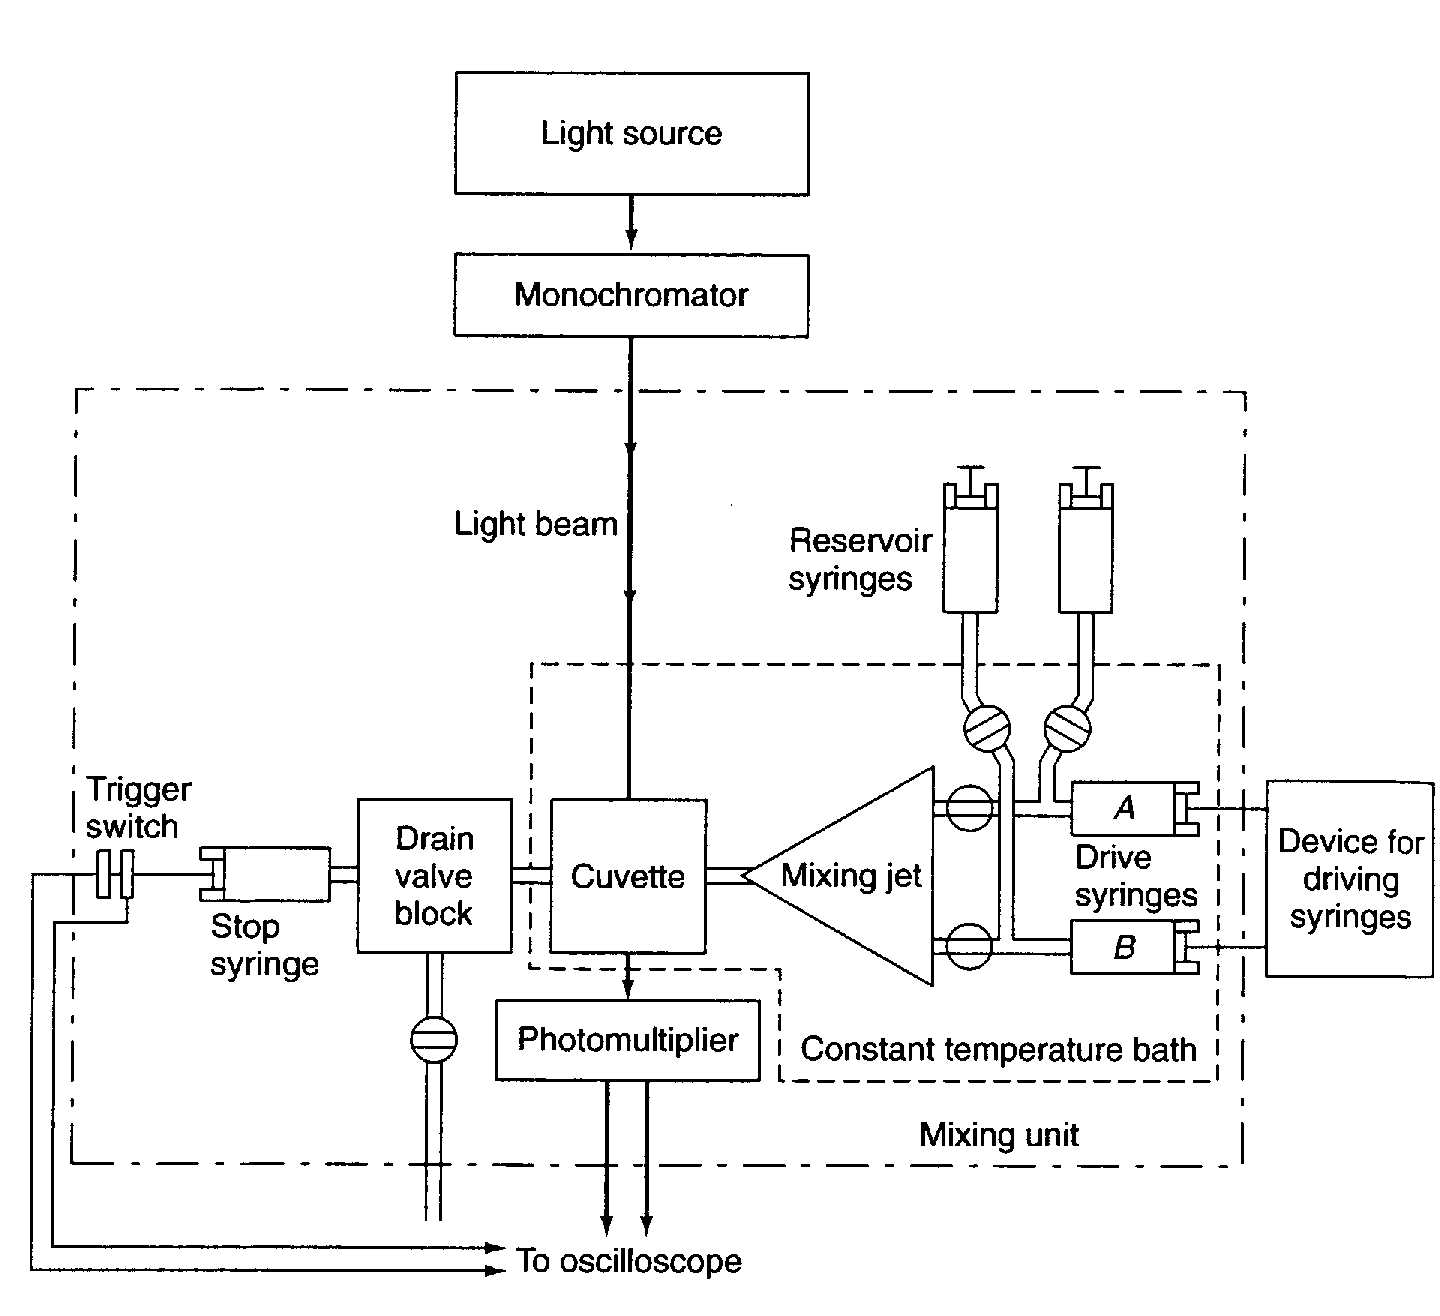
\includegraphics[scale=0.2]{fig/stopped_flow.png}
  \caption{Schematisk representation av stopped-flow utrustning}
  \label{fig:stopped-flow}
\end{figure}

Blandkammaren är termostaterad med hjälp av vattenbad som ni själva får
välja temperatur för. Ni kan börja era försök vid
rumstemperatur, temperaturintervallet ni kan arbeta inom styrs av
temperaturen av kallvattnet i husets ledningar (säg \SI{12}{\celsius})
och vattenbadets övre gräns (säg \SI{50}{\celsius}). 

Kyvettens längd är \SI{1}{\centi\metre} (vilket
tillsammans med extinktionskoefficienten  är något ni har nytta av att
veta när ni väljer koncentrationsintervall för era reaktantlösningar).

Istället för ett oscilloskåp kommer ni ha en dator med ett interface
skrivet i LabView. Handhavandet av programmet är beskrivet i
\cref{sec:handhavande}. Från varje försök kommer ni att erhålla dataserier med
absorbans som funktion av tid vid en våglängd som ni själva väljer. Dessa
tidsserier kommer sparas i form av textfiler som ni sparar på USB minne
som ni själva tar med er till labb.

\subsection{Stamlösningar}
För att bereda era reaktantlösningar kommer ni ha tillgång till följande
stamlösningar:

\begin{itemize}
\item \SI{1}{\Molar} \ce{NaClO4}
\item \SI{1}{\Molar} \ce{HClO4}
\item \SI{100}{\milli\Molar} \ce{KSCN}
\item \SI{100}{\milli\Molar} \ce{Fe(NO3)3}
\end{itemize}

\subsection{Handhavande}
\label{sec:handhavande}
Nedan finner ni en instruktion för handhavandet av
laborationsutrustningen.

\subsubsection{Förberedelser}
\begin{itemize}
\item Tänd lampan minst 5 minuter innan mätningarna.
\item Kontrollera att vattennivån i termostaten är tillräckligt hög.
Starta termostat och lägg i extern termometer.
\item Kontrollera att kylvattnet är på med hjälp av den röda flödesmätaren.
\item Sätt på kranvattnet.
\item Ställ in och invänta rätt temperatur
OBS! Vid alla mätningar och kalibreringar ska ``Stop'' vara nedtryckt på ``Start/Stop
Acquisition``. Om programmet stängs av måste kalibreringen (med dest. vatten) göras om,
tryck därför aldrig på ``Exit''. Undvik att luftbubblor kommer in i kyvetten.
\end{itemize}
\subsubsection{Kalibrering}
\begin{itemize}
\item Ställ ``Integration time'' till 2 ms.
\item Blockera strålgången med metallplåten. Tryck på ``Dark''. Ta bort metallplåten.
\item Injicera destillerat vatten. Tryck på ``Ref''.
\item Kontrollera att transmittansen och absorptionen ser ut som de bör.
\item Byt sprutor och injicera tillräckligt med reaktantlösning så att komplexet bildas i kyvetten.
\item Gå in i absorptionstfönstret och bestäm vid vilken våglängd mätningarna ska göras genom
att välja ``Peak'' i Integral/peak-menyn och ``drag-drop'':a den
vertikala linjen där ni vill mäta. Beakta att det viktiga måttet vid val
av våglängd är förhållandet mellan signal och brus (``signal-to-noise-ratio'').
\end{itemize}
\subsubsection{Mätning}
\begin{itemize}
\item Gå in på fliken ``Time mode''.
\item Välj ``As fast as possible'', ``Save to file'' och ``Use a trigger''.
\item Tryck på ``Start'' så att den gröna lampan lyser (triggern aktiveras).
\item Vinkla samtliga T-kranar nedåt.
\item Injicera snabbt in ny reaktantlösning. Håll kvar greppet i 4 sekunder.
\item Välj alltid ``Replace'' när frågerutan dyker upp (se till att
  kopiera och döpa om {\tt data.txt} ifall ni är nöjda med en körning).
\end{itemize}

%%% Local Variables:
%%% mode: latex
%%% TeX-master: "../main"
%%% ispell-local-dictionary: "swedish"
%%% End:

  \section{Dataanalys}
\label{sec:analys}
Skriv ett skript (i exmepelvis Matlab, se exempelskript i
\cref{sec:matlab-nonlinear} i Bilaga) för att passa funktionsuttryck till
era rådata. Notera att vi inte tillåter att ni kopierar in rådata från
textfilerna in i koden (det försvårar utskrift och försämrar
överskådligheten). Gör passningen både med och utan antagende om
irreversibilitet samt ``pseudo första ordningens'' kinetik (totalt 4
fall) för minst en dataserie. Funktionsuttryck får ni från härledningarna
i \cref{sec:irrev_unary,sec:rev_unary,sec:irrev_binary,sec:rev_binary}.
När ni utvärderat vilket funktionsuttryck som ger lägst osäkerhet i
bestämningen av $k_f$ kan ni använda det för analysen av övriga
mätserier.

För varje kombination av $T$ och $I$ kommer ni göra $n$ replikat. För
varje replikat får ni från kurvanpassningen en uppskattning av
hastighetskonstanten $k_i$ med en uppskattad osäkerhet
($\sigma_i$). Dessa behandlar ni sedan statistiskt genom att ta ett
viktat medelväre ($\bar{k}$) där ni använder den reciproka variansen som
vikt ($w_i$):
\begin{align}
  w_i &= \frac{1}{\sigma_i^2} \\
  \bar{k} &= \frac{\sum_i{w_i \cdot k_i}}{\sum_i{w_i}}
\end{align}
variansen ($D^2$) för det viktade medelvärdet ges då av:
\begin{align}
%  D^2 &= \frac{1}{\sum_i 1/\sigma_i^2}
   D^2 &= \frac{\sum_i w_i(k_i - \bar{k})^2}{(n - 1)\sum_j w_j}
\end{align}
vid rapportering av $\bar{k}$ anges osäkerheten konventionellt som en
standardavvikelse ($\sigma \approx \sqrt{D^2}$):
\begin{align}
  k_f &= \bar{k} \pm \sqrt{D^2}
\end{align}
vilket ger ett konfidensintervall på drygt 68\%.\footnote{
Mer finns att läsa här:
%\url{http://en.wikipedia.org/wiki/68\%E2\%80\%9395\%E2\%80\%9399.7_rule}
\url{http://en.wikipedia.org/wiki/68-95-99.7\_rule}
}. Efterföljande regressioner baserade på dessa
data gör ni då viktade med den reciproka variansen ($\frac{1}{D^2}$) som
vikt.

Nedan följer några tips:

\begin{enumerate}
\item Kom ihåg att det är ett visst
  avstånd mellan blandkammaren i stopped-flow-utrustningen och
  kyvetten vilket betyder att $t_0$ är en parameter beroende på
  flödeshastigheten ni åstadkommer vid blandingen av
  reaktantlösningarna. Ni behöver således införa den som en parameter i
  ekvationerna som används vid passningen.
\item Det kommer sannolikt behövas en fri parameter som skalar
  extinktionskoefficienten vid passningen (speciellt ifall ni använder en
  annan våglängd än $\lambda_{max}$). Denna parameter kommer då även att
  kompensera eventuellt fel i beräknad koncentration av \ce{FeSCN^{2+}}
  (vilket kan vara ganska stort pga. jonstyrkeeffekter och ev. antagande
  om irreversibilitet).
\item För att underlätta analysen kan det vara fördelaktigt att studera
  temperaturberoendet vid en given jonstyrka och {\em vice versa}:
  jonstyrkeberoendet vid en given temperatur (förslagsvis
  rumstemperatur). Att variera jonstyrka och temperatur samtidigt är
  förvisso intressant, men insamling av data och efterföljande analys
  blir för tidskrävande för denna laboration.
\item Initialgissning för hastighetskonstanten kan ni uppskatta visuellt
  från en plot av absorbans mot tid under antagandet irreversibel pseduo
  första ordningens reaktion. Då gäller: $z(t) = Ze^{-k' t} \implies k'
  \approx 1/T_{0.37}$ -- där $T_{0.37}$ är tiden det tar för 63\% av den
  begränsande reaktanten att försvinna.

% \item Hastighetsutrycket för pseudo första ordningens reaktion kan
%   linjäriseras genom att göra passningen mot logaritmen av
%   koncentrationen av den begränsande reaktanten. OLS\footnote{Ordinary
%     Least Squares} passningen är då analytisk (``closed form'') vilket
%   gör den lämplig att använda sig av för att bestämma initialgissning
%   till den icke-linjära (iterativa) passningen som behövs för ``andra
%   ordningens'' behandling.\footnote{
%   Ni kan även göra en icke-linjär passning för pseudo första ordningens
%   uttryck,   utgåendes från otransformerade data, dock kommer det
%   troligtvis endast ha en marginell effekt på erhållna parametrar.}

% \item Glöm inte att rapportera korrigering för primär kinetisk salteffekt
%   för era hastighetskonstanter.

% \item Ni behöver inte göra separata passningar för det reversibla
%   fallet. Förfarandet skiljer sig endast i den efterföljande
%   ekvationslösningen (där jämviktskonstanten nu behövs för bestämning av
%   $k_f$).
\end{enumerate}

%%% Local Variables:
%%% mode: latex
%%% TeX-master: "../main"
%%% ispell-local-dictionary: "swedish"
%%% End:

  \section{Instuderingsfrågor}
\label{sec:instudering}
Det är viktigt att ni innan laborationen har en idé om vad ni vill ta
reda på och hur ni vill gå till väga. Därför skall ni inför
laborationstillfället besvarat följande frågeställningar skriftligen:

\begin{enumerate}
\item Vad händer ifall ni försöker följa reaktionen vid för hög
  temperatur?
\item Vad händer ifall ni försöker följa reaktionen vid för hög
  jonstyrka?
\item Vad sker med jonstyrkan under reaktionsförloppet i en vattenlösning
  med stökiometriska mängder järn(III)perklorat och natriumtiocyanat med
  mycket små halter av åskådarjoner?
\item Vad är tänkbara initialkoncentrationer (dvs. vad tror ni kommer att
  fungera bra)? Dessa kan sedan justeras baserat på erhållna data.
\item Vad är jonstyrkan vid $t=0$ och $t=\infty$ för era föreslagna
  koncentrationer?
\item Vad är absorbansen vid $t=\infty$ för era föreslagna
  koncentrationer? Vid vilken transmittans tror ni att ni har bäst
  känslighet i er detektor? Vilken absorbans motsvarar det?
\end{enumerate}

%%% Local Variables:
%%% mode: latex
%%% TeX-master: "../main"
%%% ispell-local-dictionary: "swedish"
%%% End:

  \section{Laborationsrapport}
\label{sec:rapport}
Laborationsrapporten skall skickas till laboratorieassistenten en
studievecka efter laborationens genomförande. Strukturen på
laborationsrapporten ska följa den konventionella disposition som ges i 
\cref{sec:rapport-disposition}.

\subsection{Disposition}
\label{sec:rapport-disposition}
Nedan följer en lista över rubriker och vad som hör till dem för er
laborationsrapport. 
\begin{description}
  \item[Sammanfattning] \hfill \\
    Vad som på engelska är känt som ``abstract''. Här sammanfattar ni i
    ett stycke vad som gjordes och anger de viktigaste resultaten.
  \item[Inledning] \hfill \\ 
    Bakgrund till laborationen.
  \item[Teori] \hfill \\ 
    Använda teoretiska samband och eventuella härledningar.
  \item[Metod] \hfill \\ 
    Experimentell metod, experimentella förhållanden och analysförfarande.
  \item[Resultat och diskussion] \hfill \\ 
    De data ni erhållit från era analyser. Enskilda värden kan
    presenteras i flytande text, serier av värden förslagsvis i tabeller.
    Vid regressionsanalys kan en figur vara belysande. Ifall ni har
    ett stort antal figurer kan merparten av dem läggas i
    bilaga. Diskutera era resultat utifrån vad ni förväntade er och de
    approximationer ni gjort. I diskussionen finns ett visst utrymme för
    spekulationer.
  \item[Slutsatser] \hfill \\ 
    Sammanfatta det viktigaste från era resultat. Vad kan man med säkerhet
    säga (inga spekulationer)? Vad är (om något) fortfarande oklart och i
    behov av mer undersökning?
  \item[Referenser] \hfill \\
    Referenser till data/teori ni själva inte bestämt/härlett.
  \item[Bilaga - kod för analys] \hfill \\
    Kod för databehandling, kurvanpassing, figur generering (exempelvis
    Matlab skript).
  \item[Övriga bilagor] \hfill \\
    Exempelvis figurer för respektive mätserie med både rådata och
    passade kurvor. Passade parametrars värden i tabellform eller i
    etiketterna.
\end{description}

%%% Local Variables:
%%% mode: latex
%%% TeX-master: "../main"
%%% ispell-local-dictionary: "swedish"
%%% End:

  \printbibliography

\end{document}

%%% mode: latex
%%% coding: utf-8
%%% TeX-master: t
%%% LaTeX-command: "pdflatex -shell-escape"
%%% End:

